% Manuscript prepared with the LLNCS macro package (Springer), as required for
% ICITS'27 English submissions (LNNS series, at most 12 pages, anonymized review version).
\documentclass[runningheads]{llncs}
%
\usepackage[T1]{fontenc}
\usepackage{graphicx}
\usepackage{amssymb}
\usepackage{amsmath}
\usepackage{booktabs}
\usepackage{xurl}
\usepackage{xcolor}
\usepackage{flafter}
\usepackage{placeins}
\usepackage{float}
\usepackage{tikz}
\usetikzlibrary{arrows.meta,positioning,fit,calc,backgrounds}
\usepackage{pgfplots}
\pgfplotsset{compat=1.18}
\usepackage{hyperref}
\hypersetup{colorlinks=true,linkcolor=blue!50!black,citecolor=blue!50!black,urlcolor=blue!50!black}

% Palette shared by every figure
\definecolor{cDQN}{HTML}{2E6FBA}
\definecolor{cRND}{HTML}{E08E2B}
\definecolor{cSBS}{HTML}{4C9A6A}
\definecolor{cSetup}{HTML}{EEF1F5}
\definecolor{cLoop}{HTML}{EAF2FB}
\definecolor{lv0}{HTML}{1F4E8C}\definecolor{lv1}{HTML}{2E6FBA}\definecolor{lv2}{HTML}{4F8BC9}\definecolor{lv3}{HTML}{7AA6D3}\definecolor{lv4}{HTML}{A99F8E}\definecolor{lv5}{HTML}{D9A35E}\definecolor{lv6}{HTML}{E08E2B}\definecolor{lv7}{HTML}{C9731A}\definecolor{lv8}{HTML}{A85A12}
\newcommand{\cmark}{$\checkmark$}
\newcommand{\pmark}{$\circ$}

\title{A Matched-Budget Assessment of DQN Centrality Selection for Matrix Bandwidth Minimization}
\titlerunning{DQN Centrality Selection for Matrix Bandwidth Minimization}
\author{Anonymous Authors}
\institute{Affiliation omitted for review}

\begin{document}
\raggedbottom
\maketitle

\begin{abstract}
Reinforcement learning is increasingly used to choose among low-level heuristics in combinatorial optimization, yet the contribution of the learned selector is seldom separated from that of the heuristics it chooses from. This paper makes that separation for the Matrix Bandwidth Minimization Problem (MBMP) with a Deep Q-Network (DQN) that selects one of seven graph centralities to guide a randomized level-structure construction. Evaluated on 13 Harwell--Boeing instances over 30 seeds under a matched budget against random selection, the fixed centralities, the single and virtual best solvers (SBS and VBS) and Reverse Cuthill--McKee, the DQN closes only 2.2\% of the normalized SBS--VBS gap and is not consistently better than random selection. A $2\times2$ factorial ablation of selector and starting-vertex rule then locates the source of the gains, showing that a pseudo-peripheral start lowers the bandwidth of all six L-shaped meshes by 2.5 to 4.4\% under either selector while degrading the other families, and that under this start no significant difference between DQN and random selection is detected on any of the ten discriminating instances. Under a reward that favours ties over small improvements, performance is thus governed by the construction and not by the learned policy.

\keywords{Matrix bandwidth minimization \and Deep reinforcement learning \and Selection hyper-heuristics \and Graph centrality \and Algorithm selection}
\end{abstract}

\section{Introduction}

The order of the rows and columns of a sparse matrix determines how far its nonzero entries spread from the main diagonal, and this spread, the bandwidth, governs the storage and memory behaviour of many sparse linear algebra routines. In graph terms rows and columns are vertices, off-diagonal nonzeros are edges and a symmetric permutation is a vertex labeling, and the resulting Matrix Bandwidth Minimization Problem (MBMP) is NP-hard \cite{papadimitriou1976}, which is why practice relies on heuristics that range from level-structure orderings \cite{cuthill1969,gibbs1976} to metaheuristics \cite{marti2001,pinana2004,rodriguez2008,mladenovic2010}.

Because no low-cost heuristic dominates across graph families and matrix structures \cite{gonzaga2025}, it is natural to choose among several heuristics according to the instance or to the state of the search, and deep reinforcement learning (RL) has become an active way of learning such a selection rule \cite{burke2013,mazyavkina2021,kallestad2023}. The appeal of a learned selector, however, rests on the assumption that its policy chooses better than a selector that knows nothing, and this assumption has to be tested directly, since an improvement over classical baselines may come from the policy, from the diversity of the pool or from the extra budget of repeated randomized constructions.

Testing it requires yardsticks that hold the pool and the budget fixed, among which random selection isolates the value of choosing from that of diversifying, while the single best solver (SBS) and the virtual best solver (VBS) of algorithm selection \cite{kerschke2019} provide static references for a single heuristic and a per-instance oracle. We apply these yardsticks to a DQN that selects among seven graph centralities for the MBMP, building on Carneiro et al.\ \cite{carneiro2024qmch}, and ask whether learned selection adds value beyond diversification at an equal budget and, if it does not, where the improvements that the method does achieve come from.

In answering these two questions, the paper makes four contributions. First, the paper extends the Q-MCH formulation \cite{carneiro2024qmch} from two to seven centrality actions with a normalized state, a dense reward and a stabilized training loop. Second, it evaluates this selector under a matched-budget protocol with 30 seeds against random selection, every fixed centrality, the SBS, the VBS and RCM, and shows that the policy closes only 2.2\% of the normalized SBS--VBS gap. Third, a $2\times2$ factorial ablation of selector and starting-vertex rule attributes the observed gains to the construction, whose effect is beneficial on every L-shaped mesh and harmful on every other tested family, while no significant difference between the selectors is detected under the pseudo-peripheral start, although that start may also make the actions more alike. Fourth, the paper shows that the starting rule cannot remove the residual factor of about 1.5 that separates the method from RCM on the larger meshes and identifies the within-level ordering as the most plausible remaining cause, which turns a negative result on learning into an agenda for the construction.

The remainder of this paper follows the same line of argument. Section~\ref{sec:background} reviews the related work and positions the paper, Section~\ref{sec:method} describes the DQN hyper-heuristic whose value is in question, Section~\ref{sec:experiments} tests that value and locates the source of the gains, and Section~\ref{sec:conclusion} draws the conclusions.

\section{Background and Related Work}
\label{sec:background}

The question raised in the introduction draws on three bodies of work, which this section reviews in the order in which the method uses them, from the MBMP and its level-structure principle to the RL concepts behind the DQN and to heuristic and algorithm selection.

Let $G=(V,E)$ be the undirected graph of a sparse symmetric matrix and $\pi: V \rightarrow \{1,\ldots,|V|\}$ a bijective vertex labeling. The bandwidth induced by $\pi$ is $B(G,\pi)=\max_{(u,v)\in E} |\pi(u)-\pi(v)|$, and the MBMP seeks a labeling $\pi^\star \in \arg\min_{\pi} B(G,\pi)$. The Cuthill--McKee ordering \cite{cuthill1969} and its reverse variant, RCM, label the vertices along a breadth-first traversal, so that consecutive labels fill one level before the next. Because every edge then joins vertices of the same or of adjacent levels, the bandwidth is controlled by the level widths, which is why these methods start from a pseudo-peripheral vertex, of approximately maximal eccentricity, whose traversal produces many narrow levels \cite{gibbs1976}. Metaheuristics improve on such orderings at a much higher cost \cite{marti2001,pinana2004,rodriguez2008,mladenovic2010}, yet no inexpensive ordering dominates across graph classes \cite{gonzaga2025}, and this lack of dominance makes the MBMP a natural testbed for adaptive selection among cheap constructive heuristics.

Choosing among such heuristics during the search is a sequential decision problem, and reinforcement learning models it as an agent interacting with an environment, which is described by a Markov decision process $(\mathcal{S},\mathcal{A},P,R,\gamma)$, in order to maximize cumulative discounted reward, following Bellman's principle of optimality \cite{bellman1957}. Q-learning \cite{watkins1992} moves the value $Q(s,a)$ of each action towards the target $r+\gamma\max_{a'}Q(s',a')$ without a model of $P$, and Deep Q-Networks replace the table of values by a neural network $Q(s,a;\theta)$ trained with $\epsilon$-greedy exploration, replay memory and a separate target network \cite{mnih2015}.

Selection hyper-heuristics place such a learning mechanism above a set of problem-specific heuristics and choose among them according to the search context \cite{burke2013,drake2020}. Adaptive operator selection first framed this choice as a multi-armed bandit that rewards operators by their recent improvements \cite{fialho2010,auer2002}, and deep RL has since been used to learn richer selection policies \cite{mazyavkina2021,zhang2022,kallestad2023}. Whatever the learner, the value of its policy is isolated only against a selector that chooses uniformly at random from the same pool under the same budget, and algorithm selection complements this control with the SBS and the VBS, judging a selector by the fraction of the gap between them that it closes \cite{kerschke2019}, a fraction that exceeds 100\% if a selector switching heuristics beats the VBS. For the MBMP, the Q-MCH approach \cite{carneiro2024qmch} combined a DQN choosing between two centralities with a multi-centrality construction and compared the search with classical baselines, which showed that RL-guided multi-centrality search is feasible but did not separate the policy from its pool.

Table~\ref{tab:position} summarizes this positioning, in which Q-MCH is the only earlier work that joins the MBMP, centrality-guided construction and learned selection, and the present paper adds the matched baselines, the SBS--VBS gap and the factorial ablation that are needed to judge that combination.

\begin{table}[H]
\centering
\caption{Position of this paper in the literature. A \cmark{} marks a characteristic central to the work, a \pmark{} one present only in parts of the cited literature.}
\label{tab:position}
\scriptsize
\setlength{\tabcolsep}{3pt}
\begin{tabular}{lcccccc}
\toprule
Work & MBMP & \begin{tabular}[c]{@{}c@{}}Centrality\\guided\end{tabular} & \begin{tabular}[c]{@{}c@{}}Learned\\selection\end{tabular} & \begin{tabular}[c]{@{}c@{}}Matched\\baselines\end{tabular} & \begin{tabular}[c]{@{}c@{}}SBS--VBS\\gap\end{tabular} & \begin{tabular}[c]{@{}c@{}}Factorial\\ablation\end{tabular}\\
\midrule
Level-structure orderings \cite{cuthill1969,gibbs1976,gonzaga2025} & \cmark & & & & & \\
Metaheuristics \cite{marti2001,pinana2004,rodriguez2008,mladenovic2010} & \cmark & & & & & \\
Selection hyper-heuristics \cite{burke2013,drake2020,fialho2010} & & & \cmark & \pmark & & \\
Deep RL hyper-heuristics \cite{zhang2022,kallestad2023} & & & \cmark & \pmark & & \\
Algorithm selection \cite{kerschke2019} & & & \cmark & & \cmark & \\
Q-MCH \cite{carneiro2024qmch} & \cmark & \cmark & \cmark & & & \\
This paper & \cmark & \cmark & \cmark & \cmark & \cmark & \cmark \\
\bottomrule
\end{tabular}
\end{table}

\section{The DQN Selection Hyper-Heuristic}
\label{sec:method}

The selector whose value is examined in this paper follows the hyper-heuristic pattern reviewed in Section~\ref{sec:background}, with seven centrality-guided constructions as its low-level heuristics and a DQN as its learning mechanism. The decision loop that connects them is presented first, followed by the heuristics in Section~\ref{sec:heuristics} and by the learning components in Section~\ref{sec:learning}.

The method treats centrality selection as a sequential decision problem, illustrated in Fig.~\ref{fig:framework}. Seven centrality maps are computed once on the graph of the input matrix, and at each decision the DQN observes a normalized state summarizing search progress, the current and incumbent bandwidths, stagnation and the success rate of each action. The centrality it selects then guides 15 randomized constructions, whose best bandwidth yields a dense reward and updates both the search state and the network before the next decision is taken.

\begin{figure}[H]
\centering
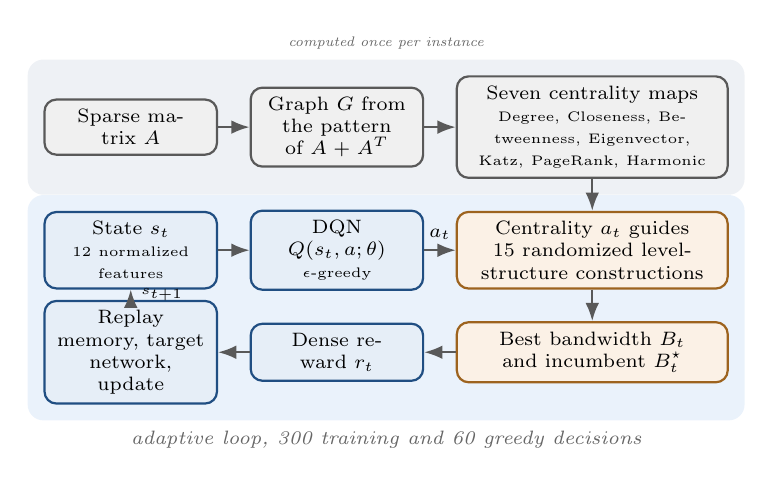
\begin{tikzpicture}[
  font=\scriptsize, >=Latex,
  blk/.style={draw=#1!70!black, fill=#1!12, rounded corners=1.5mm, thick, align=center, minimum height=7mm, text width=1.95cm, inner sep=1.2mm},
  blk/.default=gray,
  arr/.style={->, thick, draw=black!65}
]
% setup row, computed once
\node[blk=gray] (A) {Sparse matrix $A$};
\node[blk=gray, right=4mm of A] (G) {Graph $G$ from the pattern of $A+A^{T}$};
\node[blk=gray, right=4mm of G, text width=3.2cm] (C) {Seven centrality maps\\ {\tiny Degree, Closeness, Betweenness, Eigenvector, Katz, PageRank, Harmonic}};
\draw[arr] (A) -- (G);
\draw[arr] (G) -- (C);
% loop, upper row
\node[blk=cDQN, below=7mm of A] (S) {State $s_t$\\ {\tiny 12 normalized features}};
\node[blk=cDQN, right=4mm of S] (Q) {DQN $Q(s_t,a;\theta)$\\ {\tiny $\epsilon$-greedy}};
\node[blk=cRND, right=4mm of Q, text width=3.2cm] (K) {Centrality $a_t$ guides 15 randomized level-structure constructions};
% loop, lower row
\node[blk=cRND, below=4mm of K, text width=3.2cm] (B) {Best bandwidth $B_t$ and incumbent $B_t^{\star}$};
\node[blk=cDQN, left=4mm of B] (R) {Dense reward $r_t$};
\node[blk=cDQN, left=4mm of R] (U) {Replay memory, target network, update};
\draw[arr] (S) -- (Q);
\draw[arr] (Q) -- node[above]{$a_t$} (K);
\draw[arr] (C) -- (K);
\draw[arr] (K) -- (B);
\draw[arr] (B) -- (R);
\draw[arr] (R) -- (U);
\draw[arr, dashed] (U) -- node[right, font=\tiny]{$s_{t+1}$} (S);
\begin{scope}[on background layer]
\node[fill=cSetup, rounded corners=2mm, inner sep=2mm, fit=(A)(G)(C), label={[font=\tiny\itshape, text=black!60]above:computed once per instance}] {};
\node[fill=cLoop, rounded corners=2mm, inner sep=2mm, fit=(S)(K)(B)(U), label={[font=\scriptsize\itshape, text=black!60]below:adaptive loop, 300 training and 60 greedy decisions}] {};
\end{scope}
\end{tikzpicture}
\caption{The DQN centrality selection loop.}
\label{fig:framework}
\end{figure}

\subsection{Centrality-Guided Constructive Heuristics}
\label{sec:heuristics}

The low-level heuristics among which the DQN chooses are seven randomized constructions, one for each centrality listed in Fig.~\ref{fig:framework}. A construction guided by centrality $c$ samples a starting vertex with probability proportional to $c$, falling back to uniform sampling when the weights are non-finite, negative or of zero total mass, and labels the graph level by level along a breadth-first traversal from that vertex. Within each level the vertices are sorted by $c$, the top fraction $\alpha_{\mathrm{RCL}}=0.3$ forms a restricted candidate list, and the list and its complement are shuffled independently before being concatenated, so that repeated constructions differ while favouring central vertices. Each decision performs 15 constructions and returns the best bandwidth, exactly as the random and fixed baselines do.

Of these design choices, the starting vertex deserves particular attention because it interacts with the level-structure principle of Section~\ref{sec:background}. Sampling in proportion to closeness, harmonic or betweenness centrality favours vertices near the middle of the graph, whereas degree-weighted sampling is close to uniform on a mesh, and Fig.~\ref{fig:levels} shows why the central starts favoured by the first three can be harmful on mesh-like graphs. From the centre of a $5\times5$ grid the traversal has five levels of widths up to 8, whereas from a corner it has nine levels of widths at most 5, and since any ordering that labels the levels consecutively has bandwidth at most $\max_i(|L_i|+|L_{i+1}|)-1$, this bound is 15 for the central start and 8 for the peripheral one. Section~\ref{sec:ablation} returns to this mechanism and tests it by replacing the centrality-weighted start with a pseudo-peripheral vertex while keeping the centrality-guided ordering within each level.

\begin{figure}[!tb]
\centering
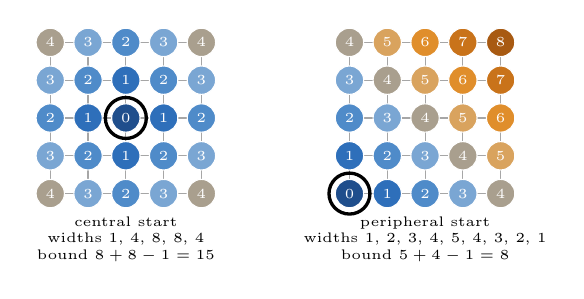
\begin{tikzpicture}[font=\scriptsize]
\begin{scope}
  \foreach \i in {0,...,4}{\foreach \j in {0,...,4}{
    \ifnum\i<4 \draw[black!35] (0.48*\i,0.48*\j) -- (0.48*\i+0.48,0.48*\j); \fi
    \ifnum\j<4 \draw[black!35] (0.48*\i,0.48*\j) -- (0.48*\i,0.48*\j+0.55); \fi }}
  \foreach \i in {0,...,4}{\foreach \j in {0,...,4}{
    \pgfmathtruncatemacro{\d}{abs(\i-2)+abs(\j-2)}
    \node[circle, fill=lv\d, draw=white, minimum size=3.6mm, inner sep=0pt, text=white] at (0.48*\i,0.48*\j) {\tiny\d}; }}
  \draw[very thick, black] (0.96,0.96) circle (2.6mm);
  \node[align=center, font=\tiny] at (0.96,-0.58) {central start\\ widths 1, 4, 8, 8, 4\\ bound $8+8-1=15$};
\end{scope}
\begin{scope}[xshift=3.8cm]
  \foreach \i in {0,...,4}{\foreach \j in {0,...,4}{
    \ifnum\i<4 \draw[black!35] (0.48*\i,0.48*\j) -- (0.48*\i+0.48,0.48*\j); \fi
    \ifnum\j<4 \draw[black!35] (0.48*\i,0.48*\j) -- (0.48*\i,0.48*\j+0.55); \fi }}
  \foreach \i in {0,...,4}{\foreach \j in {0,...,4}{
    \pgfmathtruncatemacro{\d}{\i+\j}
    \node[circle, fill=lv\d, draw=white, minimum size=3.6mm, inner sep=0pt, text=white] at (0.48*\i,0.48*\j) {\tiny\d}; }}
  \draw[very thick, black] (0,0) circle (2.6mm);
  \node[align=center, font=\tiny] at (0.96,-0.58) {peripheral start\\ widths 1, 2, 3, 4, 5, 4, 3, 2, 1\\ bound $5+4-1=8$};
\end{scope}
\end{tikzpicture}
\caption{Breadth-first levels of a $5\times5$ grid from two starting vertices (ringed).}
\label{fig:levels}
\end{figure}

\subsection{State, Reward and Training}
\label{sec:learning}

The seven constructive heuristics of Section~\ref{sec:heuristics} form the action set of the DQN, which must decide at every step which of them to run next and, to that end, observes the normalized 12-dimensional state
\[
s_t =
\left[
\tfrac{t}{T},\;
\tfrac{B_t}{B_0},\;
\tfrac{B_t^\star}{B_0},\;
\tfrac{B_0-B_t^\star}{B_0},\;
\tfrac{\tau_t}{T},\;
\rho_{1,t},\ldots,\rho_{7,t}
\right],
\]
where $T$ is the training horizon, $B_0$ the bandwidth of the original ordering, $B_t$ the bandwidth returned by the last selected heuristic, $B_t^\star$ the incumbent and $\tau_t$ the number of decisions since the last strict improvement, while $\rho_{i,t}$ is the fraction of the selections of action $i$ that strictly improved the incumbent. The state thus removes the scale of the instance and deliberately encodes nothing about the topology of the graph. The agent learns from a dense reward which, with $B^\star_{t-1}$ the incumbent before action $a_t$, is
\[
r_t =
\begin{cases}
(B^\star_{t-1}-B_t)/B_0, & B_t < B^\star_{t-1},\\
0.01, & B_t = B^\star_{t-1},\\
-0.05\min\{(B_t-B^\star_{t-1})/B_0,\,1\}, & B_t > B^\star_{t-1},
\end{cases}
\]
and which gives feedback at every step, rewarding improvements in proportion to their normalized size and ties with a small constant. Because improvements are divided by $B_0$ while ties receive a constant, an improvement earns more than a tie only when it exceeds $0.01B_0$ bandwidth units, a threshold below one unit on the \texttt{bcsstk} instances that reaches 8.2 units on the BP matrices and 18.6 units on \texttt{lshp1882}, and Section~\ref{sec:discussion} discusses the consequences of this scaling for the conclusions.

To learn from this reward, the online network uses two hidden layers of 128 ReLU units and one output per centrality, and a target network of the same architecture provides the targets $y_t = r_t + \gamma (1-d_t)\max_a Q_{\mathrm{target}}(s_{t+1},a)$, with $d_t$ flagging a terminal transition. Training uses the Smooth L1 loss and Adam with learning rate $\eta = 0.001$, discount $\gamma = 0.9$ and gradient norms clipped at 1.0, and exploration decays as $\epsilon_t=\max\{\epsilon_{\min},\epsilon_0(\epsilon_{\min}/\epsilon_0)^{t/T}\}$ with $\epsilon_0 = 1$, $\epsilon_{\min}=0.01$ and $T=300$. Transitions enter a replay buffer of capacity 10,000, learning starts once 64 transitions are available and uses mini-batches of 64, and the target network is synchronized every 25 updates. A run of 300 training and 60 greedy decisions thus consumes $360\times15=5{,}400$ constructions, the budget that the experiments hold fixed, and performs 237 gradient updates with nine target synchronizations.

\section{Computational Experiments}
\label{sec:experiments}

The experiments answer the two questions of the introduction in the order in which they arise, first whether the DQN of Section~\ref{sec:method} selects better than a selector that knows nothing under the same budget and then, because that answer is negative, where the improvements of the method come from. After the setup shared by both experiments in Section~\ref{sec:setup}, Section~\ref{sec:results} addresses the first question, Section~\ref{sec:ablation} the second, and Section~\ref{sec:discussion} weighs both answers against the threats to their validity.

\subsection{Experimental Setup}
\label{sec:setup}

Both experiments use 13 instances from the HB group of SuiteSparse \cite{davis2011,duff1989}, namely four structural engineering matrices (\texttt{bcsstk01}, \texttt{bcsstk04}, \texttt{bcsstk05} and \texttt{bcsstk06}), six L-shaped meshes (\texttt{lshp265} to \texttt{lshp1882}), two simplex-basis matrices of the BP family (\texttt{bp\_0} and \texttt{bp\_200}) and one of the SHL family (\texttt{shl\_0}). Each instance becomes a simple undirected graph, using the pattern of $A+A^{T}$ for the BP and SHL matrices, and two repository files that carry no independent information were excluded, \texttt{bcsstk02}, the complete graph $K_{66}$ with bandwidth 65 under every ordering, and \texttt{bcsstk07.mtx}, byte-identical to \texttt{bcsstk06.mtx}.

On these instances the DQN is compared with baselines that each isolate one factor. Random selection, which chooses uniformly among the seven actions at each decision, measures diversification without learning, and each fixed centrality uses a single action throughout. The VBS is the fixed centrality with the lowest mean bandwidth on each instance, a static oracle that a selector switching heuristics can exceed, and the SBS is the fixed centrality with the best mean rank over the benchmark, Katz with a mean rank of 2.50 among the seven. RCM serves as a deterministic external reference, and all stochastic methods receive the same budget of 5,400 constructions, start with $B_0$ as incumbent and use the same 30 deterministic seeds, and results are summarized by mean and standard deviation.

Because the stochastic methods share their seeds, comparisons centred on the DQN are paired and use the two-sided Wilcoxon signed-rank test \cite{wilcoxon1945} with the normal approximation, removal of zero differences and no continuity correction, with the DQN--Random and DQN--SBS $p$-values of each instance adjusted by Holm's procedure \cite{holm1979}, while the global comparison uses the Friedman test \cite{friedman1937} with tie correction. The benefit of selection is measured by $\mathrm{GapClosed}=(\mathrm{SBS}-\mathrm{DQN})/(\mathrm{SBS}-\mathrm{VBS})$, computed on the mean normalized bandwidth $B/B_0$ because bandwidths differ by orders of magnitude across instances.

Finally, every run was a job on a fresh GitHub-hosted virtual machine configured as in Table~\ref{tab:env}, whose physical processor is assigned at provisioning, so times serve only as paired estimates. In the ablation jobs of Section~\ref{sec:ablation}, where the DQN and Random shared a machine, the DQN needed about 5.4\% and 6.2\% more time than Random with the centrality-based and the pseudo-peripheral start, so learning costs little compared with the constructions.

\begin{table}[H]
\centering
\caption{Hardware and software used in all experiments.}
\label{tab:env}
\scriptsize
\setlength{\tabcolsep}{4pt}
\begin{tabular}{llll}
\toprule
\multicolumn{2}{c}{Hardware} & \multicolumn{2}{c}{Software}\\
\cmidrule(lr){1-2}\cmidrule(lr){3-4}
Platform & GitHub-hosted runner & Operating system & Ubuntu 24.04\\
Architecture & x64 virtual machine & Python & CPython 3.11.17\\
Processor & 4 vCPUs, model varies & PyTorch & 2.14.1, CPU only\\
Memory & 16 GB RAM & NetworkX & 3.6.1\\
Storage & 14 GB SSD & NumPy, SciPy & 2.4.6, 1.17.1\\
GPU & none & Pandas & 3.0.6\\
\bottomrule
\end{tabular}
\end{table}

\subsection{The Learned Selector Against the Portfolio}
\label{sec:results}

The first question presupposes that the choice of centrality matters, and Table~\ref{tab:mainresults} confirms that it does. The best fixed centrality changes with the instance, Eigenvector being best on \texttt{bcsstk01} and \texttt{shl\_0}, Harmonic on \texttt{bp\_0}, Closeness on \texttt{bp\_200}, Degree on the smaller meshes and Katz on most of the larger ones, whereas \texttt{bcsstk04}, \texttt{bcsstk05} and \texttt{bcsstk06} are not discriminating, since every stochastic method returns $B_0$ on all seeds.

\begin{table}[!tb]
\centering
\caption{Mean bandwidth $\pm$ standard deviation over 30 seeds. RCM is deterministic.}
\label{tab:mainresults}
\scriptsize
\setlength{\tabcolsep}{2.6pt}
\begin{tabular}{lrrrrrrrr}
\toprule
Instance & $|V|$ & $|E|$ & $B_0$ & RCM & DQN & Random & SBS (Katz) & VBS\\
\midrule
bcsstk01 & 48 & 176 & 35 & 26 & $26.20\pm0.55$ & $26.43\pm0.50$ & $25.97\pm0.49$ & $\mathbf{25.83\pm0.65}$\\
bcsstk04 & 132 & 1758 & 47 & 54 & $47.00\pm0.00$ & $47.00\pm0.00$ & $47.00\pm0.00$ & $47.00\pm0.00$\\
bcsstk05 & 153 & 1135 & 28 & 24 & $28.00\pm0.00$ & $28.00\pm0.00$ & $28.00\pm0.00$ & $28.00\pm0.00$\\
bcsstk06 & 420 & 3720 & 47 & 50 & $47.00\pm0.00$ & $47.00\pm0.00$ & $47.00\pm0.00$ & $47.00\pm0.00$\\
bp\_0 & 822 & 3260 & 820 & 422 & $573.43\pm3.20$ & $572.93\pm4.12$ & $572.93\pm3.19$ & $\mathbf{572.70\pm3.10}$\\
bp\_200 & 822 & 3788 & 820 & 506 & $600.57\pm4.63$ & $\mathbf{597.30\pm5.29}$ & $598.07\pm3.23$ & $597.63\pm5.08$\\
lshp265 & 265 & 744 & 256 & 18 & $25.00\pm0.59$ & $25.00\pm0.64$ & $25.20\pm0.41$ & $\mathbf{24.40\pm0.56}$\\
lshp406 & 406 & 1155 & 394 & 22 & $31.37\pm0.56$ & $31.27\pm0.58$ & $31.83\pm0.53$ & $\mathbf{30.67\pm0.48}$\\
lshp1009 & 1009 & 2928 & 991 & 34 & $51.23\pm0.57$ & $50.80\pm0.76$ & $\mathbf{50.40\pm0.50}$ & $\mathbf{50.40\pm0.62}$\\
lshp1270 & 1270 & 3699 & 1250 & 38 & $58.07\pm0.94$ & $57.63\pm0.61$ & $\mathbf{56.93\pm0.52}$ & $\mathbf{56.93\pm0.52}$\\
lshp1561 & 1561 & 4560 & 1539 & 42 & $64.27\pm0.83$ & $64.27\pm0.83$ & $\mathbf{63.50\pm0.51}$ & $\mathbf{63.50\pm0.51}$\\
lshp1882 & 1882 & 5511 & 1858 & 46 & $70.93\pm0.91$ & $70.73\pm0.83$ & $\mathbf{70.03\pm0.56}$ & $\mathbf{70.03\pm0.56}$\\
shl\_0 & 663 & 1682 & 661 & 424 & $493.33\pm9.52$ & $497.80\pm8.09$ & $501.17\pm7.15$ & $\mathbf{485.00\pm6.46}$\\
\bottomrule
\end{tabular}
\end{table}

Whether the DQN exploits this variation is first assessed by rank. A Friedman test over the DQN, Random and the seven fixed centralities rejects equal performance ($\chi_F^2=52.21$, $p=1.53\times10^{-8}$), but the difference does not favour the learned selector, since Degree (3.27), Katz (3.31) and Random (3.35) all rank ahead of the DQN (4.08). The paired comparisons of Table~\ref{tab:posthoc} on the ten discriminating instances confirm this ordering, since after Holm correction the DQN is significantly worse than Random on \texttt{bp\_200} and \texttt{lshp1009} and not significantly different elsewhere, while against the SBS it is significantly worse on \texttt{bp\_200} and the four largest meshes and significantly better on \texttt{lshp406} and \texttt{shl\_0}, so the policy neither beats random choice nor reliably beats the best single heuristic.

\begin{table}[!tb]
\centering
\caption{Paired comparisons from the DQN perspective, with Holm-adjusted Wilcoxon $p$-values $p_H$ in bold when below 0.05.}
\label{tab:posthoc}
\scriptsize
\setlength{\tabcolsep}{5pt}
\begin{tabular}{lrrrr}
\toprule
& \multicolumn{2}{c}{vs Random} & \multicolumn{2}{c}{vs SBS (Katz)}\\
\cmidrule(lr){2-3}\cmidrule(lr){4-5}
Instance & W/T/L & $p_H$ & W/T/L & $p_H$\\
\midrule
bcsstk01 & 10/15/5 & $0.179$ & 4/16/10 & $0.179$\\
bp\_0 & 19/0/11 & $0.959$ & 10/3/17 & $0.852$\\
bp\_200 & 7/1/22 & $\mathbf{0.022}$ & 8/3/19 & $\mathbf{0.036}$\\
lshp265 & 8/15/7 & $0.953$ & 8/20/2 & $0.116$\\
lshp406 & 5/17/8 & $0.499$ & 14/14/2 & $\mathbf{0.006}$\\
lshp1009 & 2/14/14 & $\mathbf{0.003}$ & 2/8/20 & $\mathbf{<0.001}$\\
lshp1270 & 6/8/16 & $0.056$ & 1/7/22 & $\mathbf{<0.001}$\\
lshp1561 & 10/10/10 & $1.000$ & 3/8/19 & $\mathbf{0.001}$\\
lshp1882 & 9/8/13 & $0.465$ & 1/7/22 & $\mathbf{<0.001}$\\
shl\_0 & 18/1/11 & $0.076$ & 22/2/6 & $\mathbf{0.001}$\\
\bottomrule
\end{tabular}
\end{table}

Measuring the DQN against the VBS, which is strictly better than the DQN on every discriminating instance, leads to the same conclusion, and Fig.~\ref{fig:gap}, which expresses each method as its relative excess over the VBS, shows no systematic advantage for the learned selector. The DQN lies between 0.1 and 2.5\% above the VBS, Random spans a similar range and is closer to the VBS on six of the ten instances, and the SBS coincides with the VBS on the four largest meshes but falls more than 3\% behind on \texttt{lshp265}, \texttt{lshp406} and \texttt{shl\_0}. On the mean normalized bandwidth the scores are 0.48323 for the DQN, 0.48329 for the SBS and 0.48058 for the VBS, so the learned selector closes only 2.2\% of the SBS--VBS gap.

\begin{figure}[!tb]
\centering
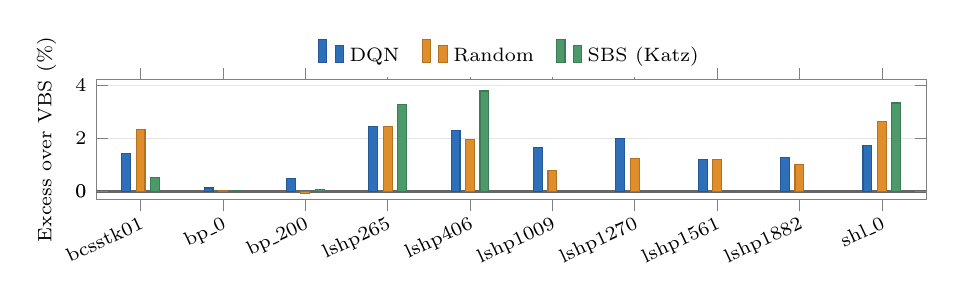
\begin{tikzpicture}
\begin{axis}[
  width=\textwidth, height=3.1cm,
  ybar, bar width=3.2pt,
  ymin=-0.3, ymax=4.2,
  ylabel={Excess over VBS (\%)}, ylabel style={font=\scriptsize},
  symbolic x coords={bcsstk01,bp\_0,bp\_200,lshp265,lshp406,lshp1009,lshp1270,lshp1561,lshp1882,shl\_0},
  xtick=data, xticklabel style={font=\scriptsize, rotate=25, anchor=north east, inner sep=1pt},
  yticklabel style={font=\scriptsize},
  ymajorgrids, grid style={black!10},
  legend style={font=\scriptsize, at={(0.5,1.02)}, anchor=south, legend columns=3, draw=none, /tikz/every even column/.append style={column sep=6pt}},
  enlarge x limits=0.06, axis line style={black!50}, tick style={black!50},
  extra y ticks={0}, extra y tick style={grid style={black!60, thick}}
]
\addplot[fill=cDQN, draw=cDQN!80!black] coordinates {(bcsstk01,1.43) (bp\_0,0.13) (bp\_200,0.49) (lshp265,2.46) (lshp406,2.28) (lshp1009,1.65) (lshp1270,2.00) (lshp1561,1.21) (lshp1882,1.29) (shl\_0,1.72)};
\addplot[fill=cRND, draw=cRND!80!black] coordinates {(bcsstk01,2.32) (bp\_0,0.04) (bp\_200,-0.06) (lshp265,2.46) (lshp406,1.96) (lshp1009,0.79) (lshp1270,1.23) (lshp1561,1.21) (lshp1882,1.00) (shl\_0,2.64)};
\addplot[fill=cSBS, draw=cSBS!80!black] coordinates {(bcsstk01,0.54) (bp\_0,0.04) (bp\_200,0.07) (lshp265,3.28) (lshp406,3.78) (lshp1009,0) (lshp1270,0) (lshp1561,0) (lshp1882,0) (shl\_0,3.33)};
\legend{DQN, Random, SBS (Katz)}
\end{axis}
\end{tikzpicture}
\caption{Relative excess of mean bandwidth over the VBS on the discriminating instances.}
\label{fig:gap}
\end{figure}

This aggregate must be read with care, because normalizing by $B_0$ makes \texttt{shl\_0} account for about 69\% of the gap, so the 2.2\% of the DQN is a gain on that instance almost cancelled by losses elsewhere. Computed from the means of Table~\ref{tab:mainresults}, Random scores about 0.48381, a gap closure of about $-19\%$, so neither selector captures a meaningful share of the benefit of per-instance selection. The greedy phase that follows training adds little either, since its 60 decisions found a lower bandwidth than the 300 training decisions in only 20 of the 390 runs, and in none on \texttt{lshp1009} or \texttt{lshp1561}. The answer to the first question is therefore negative, and Table~\ref{tab:mainresults} already hints at where the answer to the second lies, since all stochastic methods, although well below $B_0$, are dominated by RCM on nine of the ten discriminating instances, often by a wide margin.

\subsection{Factorial Ablation of Selector and Starting Vertex}
\label{sec:ablation}

The dominance of RCM points to the construction rather than to the selector, since on the four largest meshes RCM reaches 34, 38, 42 and 46 against DQN means of 51.23, 58.07, 64.27 and 70.93. Since RCM starts from a pseudo-peripheral vertex while our constructions favour central starts, we crossed DQN and Random with the centrality-weighted start and a pseudo-peripheral (PP) start, obtaining the variants DQN, DQN-PP, Random and Random-PP, with every other component unchanged, and ran them with 30 paired seeds on the six meshes and on \texttt{bcsstk01}, \texttt{bp\_0}, \texttt{bp\_200} and \texttt{shl\_0}. Table~\ref{tab:grid} lists the means together with the paired comparison of DQN-PP and Random-PP.

\begin{table}[!tb]
\centering
\caption{Factorial ablation over 30 paired seeds. W/T/L and $p_H$ compare DQN-PP with Random-PP.}
\label{tab:grid}
\scriptsize
\setlength{\tabcolsep}{4pt}
\begin{tabular}{lrrrrrr}
\toprule
Instance & DQN & DQN-PP & Random & Random-PP & W/T/L & $p_H$\\
\midrule
bcsstk01 & $26.20\pm0.55$ & $28.10\pm0.61$ & $26.43\pm0.50$ & $28.23\pm0.57$ & 8/17/5 & 0.317\\
bp\_0 & $573.43\pm3.20$ & $628.97\pm3.01$ & $572.93\pm4.12$ & $628.73\pm3.07$ & 10/5/15 & 0.715\\
bp\_200 & $600.57\pm4.63$ & $632.60\pm6.22$ & $597.30\pm5.29$ & $631.87\pm5.76$ & 14/1/15 & 0.475\\
lshp265 & $25.00\pm0.59$ & $\mathbf{23.93\pm0.25}$ & $25.00\pm0.64$ & $\mathbf{23.90\pm0.40}$ & 2/25/3 & 0.655\\
lshp406 & $31.37\pm0.56$ & $\mathbf{30.00\pm0.37}$ & $31.27\pm0.58$ & $\mathbf{30.03\pm0.32}$ & 4/23/3 & 0.705\\
lshp1009 & $51.23\pm0.57$ & $\mathbf{49.30\pm0.53}$ & $50.80\pm0.76$ & $\mathbf{49.43\pm0.50}$ & 9/15/6 & 0.346\\
lshp1270 & $58.07\pm0.94$ & $\mathbf{55.93\pm0.52}$ & $57.63\pm0.61$ & $\mathbf{55.83\pm0.46}$ & 5/17/8 & 0.499\\
lshp1561 & $64.27\pm0.83$ & $\mathbf{62.30\pm0.53}$ & $64.27\pm0.83$ & $\mathbf{62.20\pm0.48}$ & 4/18/8 & 0.439\\
lshp1882 & $70.93\pm0.91$ & $\mathbf{69.00\pm0.59}$ & $70.73\pm0.83$ & $\mathbf{68.97\pm0.49}$ & 4/18/8 & 0.934\\
shl\_0 & $493.33\pm9.52$ & $542.83\pm6.30$ & $497.80\pm8.09$ & $543.63\pm5.87$ & 12/4/14 & 0.731\\
\bottomrule
\end{tabular}
\end{table}

The effect of the PP start, shown in Fig.~\ref{fig:ablation} as a relative change in mean bandwidth under each selector, is strong and family-dependent. On every mesh the PP start lowers the bandwidth, by 2.7 to 4.4\% under the DQN and by 2.5 to 4.4\% under Random, as the level-width argument of Fig.~\ref{fig:levels} predicts, whereas on \texttt{bcsstk01}, the BP matrices and \texttt{shl\_0} it raises the bandwidth by 5.3 to 10.0\% under both selectors. The two bars of each instance are almost equal, and no significant difference between DQN-PP and Random-PP is detected on any instance ($p_H\geq0.317$). The improvement on the meshes is therefore produced by the starting rule, which the learned selector neither creates nor amplifies, although the PP start also removes one of the two places where the centrality acts and may thus bring the seven actions closer to one another.

\begin{figure}[H]
\centering
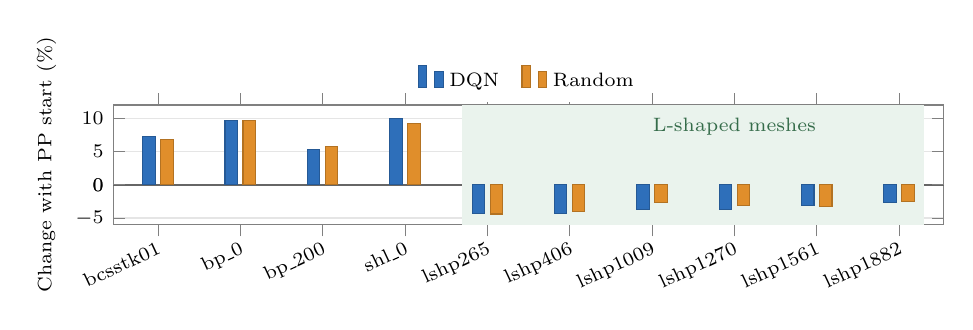
\begin{tikzpicture}
\begin{axis}[
  width=\textwidth, height=3.1cm,
  ybar, bar width=4.5pt,
  ymin=-6, ymax=12,
  ylabel={Change with PP start (\%)}, ylabel style={font=\scriptsize},
  symbolic x coords={bcsstk01,bp\_0,bp\_200,shl\_0,lshp265,lshp406,lshp1009,lshp1270,lshp1561,lshp1882},
  xtick=data, xticklabel style={font=\scriptsize, rotate=25, anchor=north east, inner sep=1pt},
  yticklabel style={font=\scriptsize},
  ymajorgrids, grid style={black!10},
  legend style={font=\scriptsize, at={(0.5,1.02)}, anchor=south, legend columns=2, draw=none, /tikz/every even column/.append style={column sep=6pt}},
  enlarge x limits=0.06, axis line style={black!50}, tick style={black!50},
  extra y ticks={0}, extra y tick style={grid style={black!60, thick}},
  clip=false
]
\fill[cSBS!12] ([xshift=-9pt]axis cs:lshp265,-6) rectangle ([xshift=9pt]axis cs:lshp1882,12);
\addplot[fill=cDQN, draw=cDQN!80!black] coordinates {(bcsstk01,7.25) (bp\_0,9.69) (bp\_200,5.33) (shl\_0,10.03) (lshp265,-4.28) (lshp406,-4.37) (lshp1009,-3.77) (lshp1270,-3.69) (lshp1561,-3.07) (lshp1882,-2.72)};
\addplot[fill=cRND, draw=cRND!80!black] coordinates {(bcsstk01,6.81) (bp\_0,9.74) (bp\_200,5.79) (shl\_0,9.21) (lshp265,-4.40) (lshp406,-3.97) (lshp1009,-2.70) (lshp1270,-3.12) (lshp1561,-3.22) (lshp1882,-2.49)};
\legend{DQN, Random}
\node[font=\scriptsize, text=cSBS!70!black, anchor=north] at (axis cs:lshp1270,11.5) {L-shaped meshes};
\end{axis}
\end{tikzpicture}
\caption{Change in mean bandwidth caused by the pseudo-peripheral (PP) start. Negative values are improvements.}
\label{fig:ablation}
\end{figure}

The starting rule does not, however, close the gap to RCM. On the four largest meshes DQN-PP still reaches 49.30, 55.93, 62.30 and 69.00 against RCM values of 34, 38, 42 and 46, a residual factor between 1.45 and 1.50. Since the PP start even worsens the BP and SHL matrices, on which RCM is far better although it also starts from a pseudo-peripheral vertex, the start cannot be the whole explanation, and the most plausible remaining cause lies inside the levels, where our construction sorts each level globally by centrality and shuffles it, whereas Cuthill--McKee labels the vertices of a level in the order of their parents and thus keeps neighbouring vertices close.

\subsection{Discussion and Threats to Validity}
\label{sec:discussion}

Taken together, the two experiments carry a methodological lesson, since without random selection at a matched budget the mesh improvements would have been easy to credit to learning. Several limitations bound how far this lesson extends. The most important is the reward scale of Section~\ref{sec:learning}, under which a tie earns more than any improvement smaller than $0.01B_0$, so on the larger meshes and the BP matrices the agent is rewarded more for reproducing the incumbent than for improving it by a few units, and the negative result on learning therefore holds for this reward and should not be extended to learned selection in general. The yardsticks have their own limits, since the VBS is static, the SBS is chosen by mean rank while the gap is measured on normalized bandwidth, the normalization by the file bandwidth $B_0$ lets \texttt{shl\_0} dominate the gap, and the absence of significant differences in Tables~\ref{tab:posthoc} and \ref{tab:grid} is not evidence of equivalence, since no equivalence test was performed. Because actions do not modify the graph, the formulation is also close to a contextual bandit, so the untested bandit selectors UCB1 \cite{auer2002} and adaptive pursuit \cite{fialho2010} are natural comparators. Finally, each DQN is trained on a single instance and performs only 237 gradient updates, within a benchmark of 13 instances from four families.

\section{Conclusion}
\label{sec:conclusion}

This paper asked whether a DQN that selects among seven centrality-guided constructive heuristics contributes to solving the MBMP, and the matched-budget experiments answered that in the configuration tested it does not beat random selection, while the clearest improvement comes from a pseudo-peripheral start that benefits both selectors on the meshes and degrades the other families.

Because this configuration uses a reward that favours ties over small improvements, the finding is that improving the constructive mechanism mattered more here than replacing random selection by deep RL, and not that learned selection cannot help. The broader lesson is that random selection at an equal budget, together with the SBS--VBS gap, should accompany any claim about learned heuristic selection, and that the next steps for this method are to test parent-preserving within-level orderings inspired by Cuthill--McKee, to rescale the reward so that every strict improvement outweighs a tie, and then to compare the DQN with bandit selectors and train it across instances before any increase in model complexity is considered.


\begin{credits}
\subsubsection{\ackname}
Omitted for review.
% Camera-ready version:
% This research was financed in part by the Conselho Nacional de Desenvolvimento Cient\'{\i}fico e Tecnol\'{o}gico -- CNPq (304043/2025-7) and Funda\c{c}\~{a}o Carlos Chagas Filho de Amparo \`{a} Pesquisa do Estado do Rio de Janeiro -- FAPERJ (E-26/204.211/2025).
\subsubsection{Declaration of Generative AI in Scientific Writing.}
During the preparation of this manuscript, the authors used OpenAI ChatGPT and Anthropic Claude to assist with language refinement, readability, manuscript organization and consistency checking. All AI-assisted content was critically reviewed and validated by the authors, who take full responsibility for the final content of the manuscript.
\end{credits}

\bibliographystyle{splncs04}
\bibliography{references}

\end{document}